\documentclass{article}

\usepackage[T1]{fontenc} 
\usepackage[ngerman]{babel}
\usepackage{graphicx}
\bibliography{literatur}
\usepackage{listings}

\usepackage{xcolor}
\definecolor{codegreen}{rgb}{0,0.6,0}
\definecolor{codegray}{rgb}{0.5,0.5,0.5}
\definecolor{codeorange}{rgb}{1,0.49,0}
\definecolor{backcolour}{rgb}{0.95,0.95,0.96}

\lstdefinestyle{mystyle}{
	backgroundcolor=\color{backcolour},   
	commentstyle=\color{codegray},
	keywordstyle=\color{codeorange},
	numberstyle=\tiny\color{codegray},
	stringstyle=\color{codegreen},
	basicstyle=\ttfamily\footnotesize,
	breakatwhitespace=false,         
	breaklines=true,                 
	captionpos=b,                    
	keepspaces=true,                 
	numbers=left,                    
	numbersep=5pt,                  
	showspaces=false,                
	showstringspaces=false,
	showtabs=false,                  
	tabsize=2,
	xleftmargin=10pt,
}

\lstset{style=mystyle}
	
\begin{document}
\newpage

\section{Implementation in Streamlit}
% In this section we describe the Haar Cascade classifier app using Streamlit
% dashboard.



\lstinputlisting[caption=app.py, language=Python]{../../app.py}
\lstinputlisting[caption=app.py, language=Python]{../../pki_a22_app/haarcascades/haarcascades.py}
\newpage
\begin{figure}
	\centering
	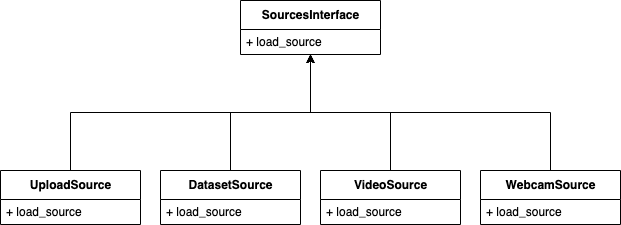
\includegraphics[scale=0.5]{input_sources.png}
	\caption{UML Diagramm für unterschiedliche Source-Typen}
\end{figure}
\lstinputlisting[caption=app.py, language=Python]{../../pki_a22_app/dashboard/sources.py}
\lstinputlisting[caption=app.py, language=Python]{../../pki_a22_app/dashboard/source_upload.py}
\lstinputlisting[caption=app.py, language=Python]{../../pki_a22_app/dashboard/source_dataset.py}
\lstinputlisting[caption=app.py, language=Python]{../../pki_a22_app/dashboard/source_video.py}
\lstinputlisting[caption=app.py, language=Python]{../../pki_a22_app/dashboard/source_webcam.py}
\lstinputlisting[caption=app.py, language=Python]{../../pki_a22_app/utils/file_loader.py}


\end{document}

 